% ECE4900W Communicating Engineering Solutions
% Author: Arturo Salinas-Aguayo <artjsalina5@uconn.edu>
\documentclass{beamer}
%\setbeameroption{show only notes}
\usetheme{Warsaw}
\usecolortheme{dolphin}
\usefonttheme{professionalfonts}
\setbeamertemplate{navigation symbols}{}
\setbeamertemplate{footline}[frame number]
\usepackage{graphicx}
\usepackage{biblatex}
\addbibresource{references.bib}
\graphicspath{{../../images/}}

\title[Safe Nuclear Power]{Safe Nuclear Power: Instrumentation, Human Oversight, and Infrastructure Transition}
\subtitle{ECE 4900W – Summer 2025}
\author[Arturo Salinas]{Arturo Salinas-Aguayo}
\institute[UConn]{University of Connecticut\\College of Engineering}
\date{\today}

\begin{document}

\begin{frame}
  \titlepage
  \note{Welcome. This presentation explores the technological, ethical, and infrastructural dimensions of nuclear power in the modern world. We will cover lessons from historic accidents, instrumentation, human-machine interface design, and current innovations. Each story reveals both vulnerability and resilience.}
\end{frame}

\begin{frame}{Outline}
  \tableofcontents
   \note{I will be going through some motivation as to why nuclear power is still safe, explain a little bit about how the fission process works and the instrumentation that is used to control the reaction. I will then go on to emphasize the broader impacts and tell the story as to why nuclear power has not been as widely adopted as it could have been. I will discuss the improvements to human factors engineering because of these, and talk about the economic, environmental, and societal impacts that these accidents have had on the nuclear industry as a whole.}
\end{frame}

\section{Introduction}

\begin{frame}
  \begin{columns}
    \column{0.48\textwidth}
  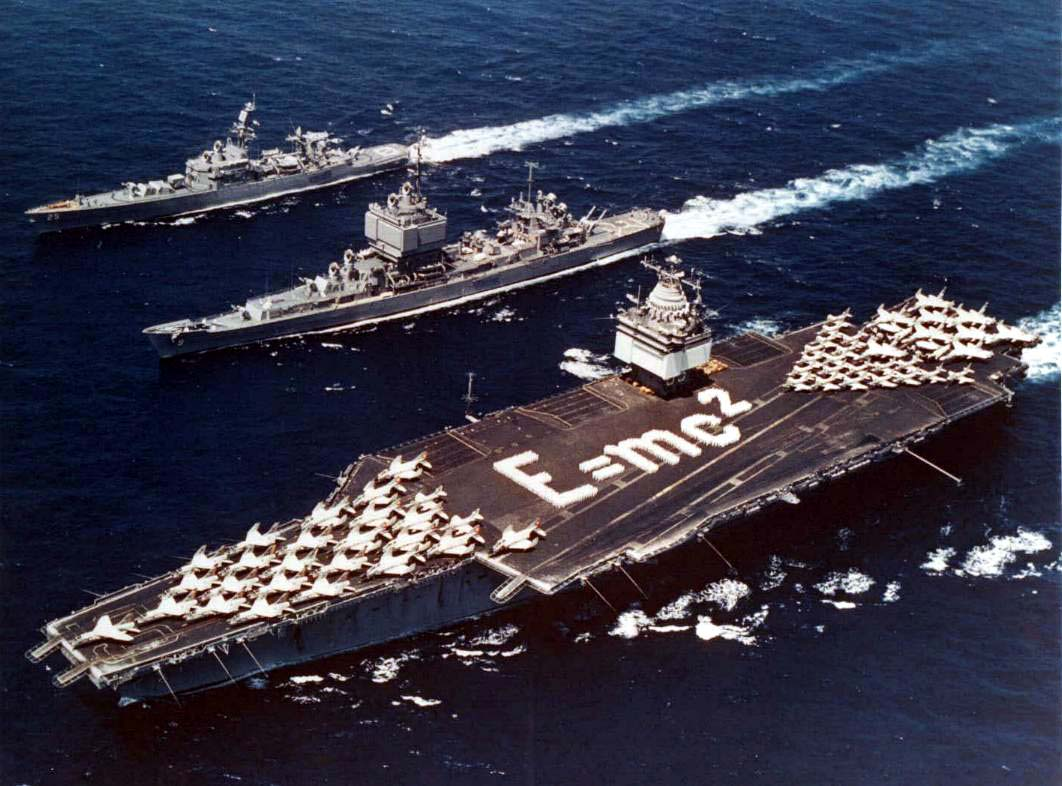
\includegraphics[width=\textwidth]{enterprise}
    \column{0.48\textwidth}
    \begin{itemize}
      \item Nuclear power plants are designed to be safe and efficient.
      \item Instrumentation plays a critical role in monitoring and control.
      \item Human oversight is essential for safe operation.
    \end{itemize}
  \note{I've been hearing a lot of misunderstanding when it comes to this photograph taken on july 31, 1964 with the uss enterprise, the uss long beach, and the uss bainbridge. I've heard  generally think that the sailors aboard irrelevantly spelled $e = mc^2$. This is just a response out of ignorance however. The formula refers to the fact that as the mass of the fuel increases, the potential for it to create energy is proprotional with that multiplied times the speed of light squared. This was a demonstration of force and showing the world the US Navy's capabilities in the nuclear age. The Enterprise was the first nuclear-powered aircraft carrier with 8 submarine reactors. The uss long beach and uss bainbridge were also powered by dual surface developed reactors.}
\end{columns}
\end{frame}

\begin{frame}{Motivation}
  \subsubsection*{Why Nuclear Now?}
  \begin{itemize}
    \item High energy density and steady base-load power
    \item Nearly zero emissions, independent of weather
    \item Risks of failure—catastrophic if unmanaged
  \end{itemize}
  \note{Despite fears, nuclear remains one of the most efficient and clean energy sources. But it requires precision and care at every level.}
\end{frame}

\begin{frame}{The Fission Process}
  \subsubsection*{Where It All Begins}
  \begin{equation}
    ^{235}\text{U} + ^{1}\text{n} \rightarrow ^{92}\text{Kr} + ^{141}\text{Ba} + 3^{1}\text{n} + \text{Energy} \approx 200~\text{MeV}
  \end{equation}
  \begin{itemize}
    \item A neutron collides with uranium-235, causing it to split
    \item Releases energy and more neutrons → possible chain reaction
  \end{itemize}
  \note{This is the reaction that drives nuclear power. The energy release is immense, but so is the potential for instability if left uncontrolled.}
\end{frame}

\begin{frame}{Reactivity and Control}
  \subsubsection*{Choreographing Neutrons}
  \begin{equation}
    \rho = \frac{k_{\text{eff}} - 1}{k_{\text{eff}}}
  \end{equation}
  \begin{itemize}
    \item $k_{\text{eff}}$: effective neutron multiplication factor
    \item $\rho > 0$: supercritical (power increases)
    \item $\rho = 0$: critical (steady power)
    \item $\rho < 0$: subcritical (power decreases)
  \end{itemize}
  \note{This is our friend Keff. The effective multiplication factor. The effective multiplication factor is just a measure of the average amount of thermal neutrons produced in one neutron lifecycle. The ratio of keff - 1 divided by keff forms a measurement called reactivity. A critical reactor has a keff of 1, a subcritical reactor has a keff of less than 1, and a supercritical reactor has a keff of greater than 1. }
\end{frame}

\section{Reactor Designs and Sensors}

\begin{frame}{Types of Reactors and PWR Instrumentation}
  \begin{columns}
    \column{0.48\textwidth}
    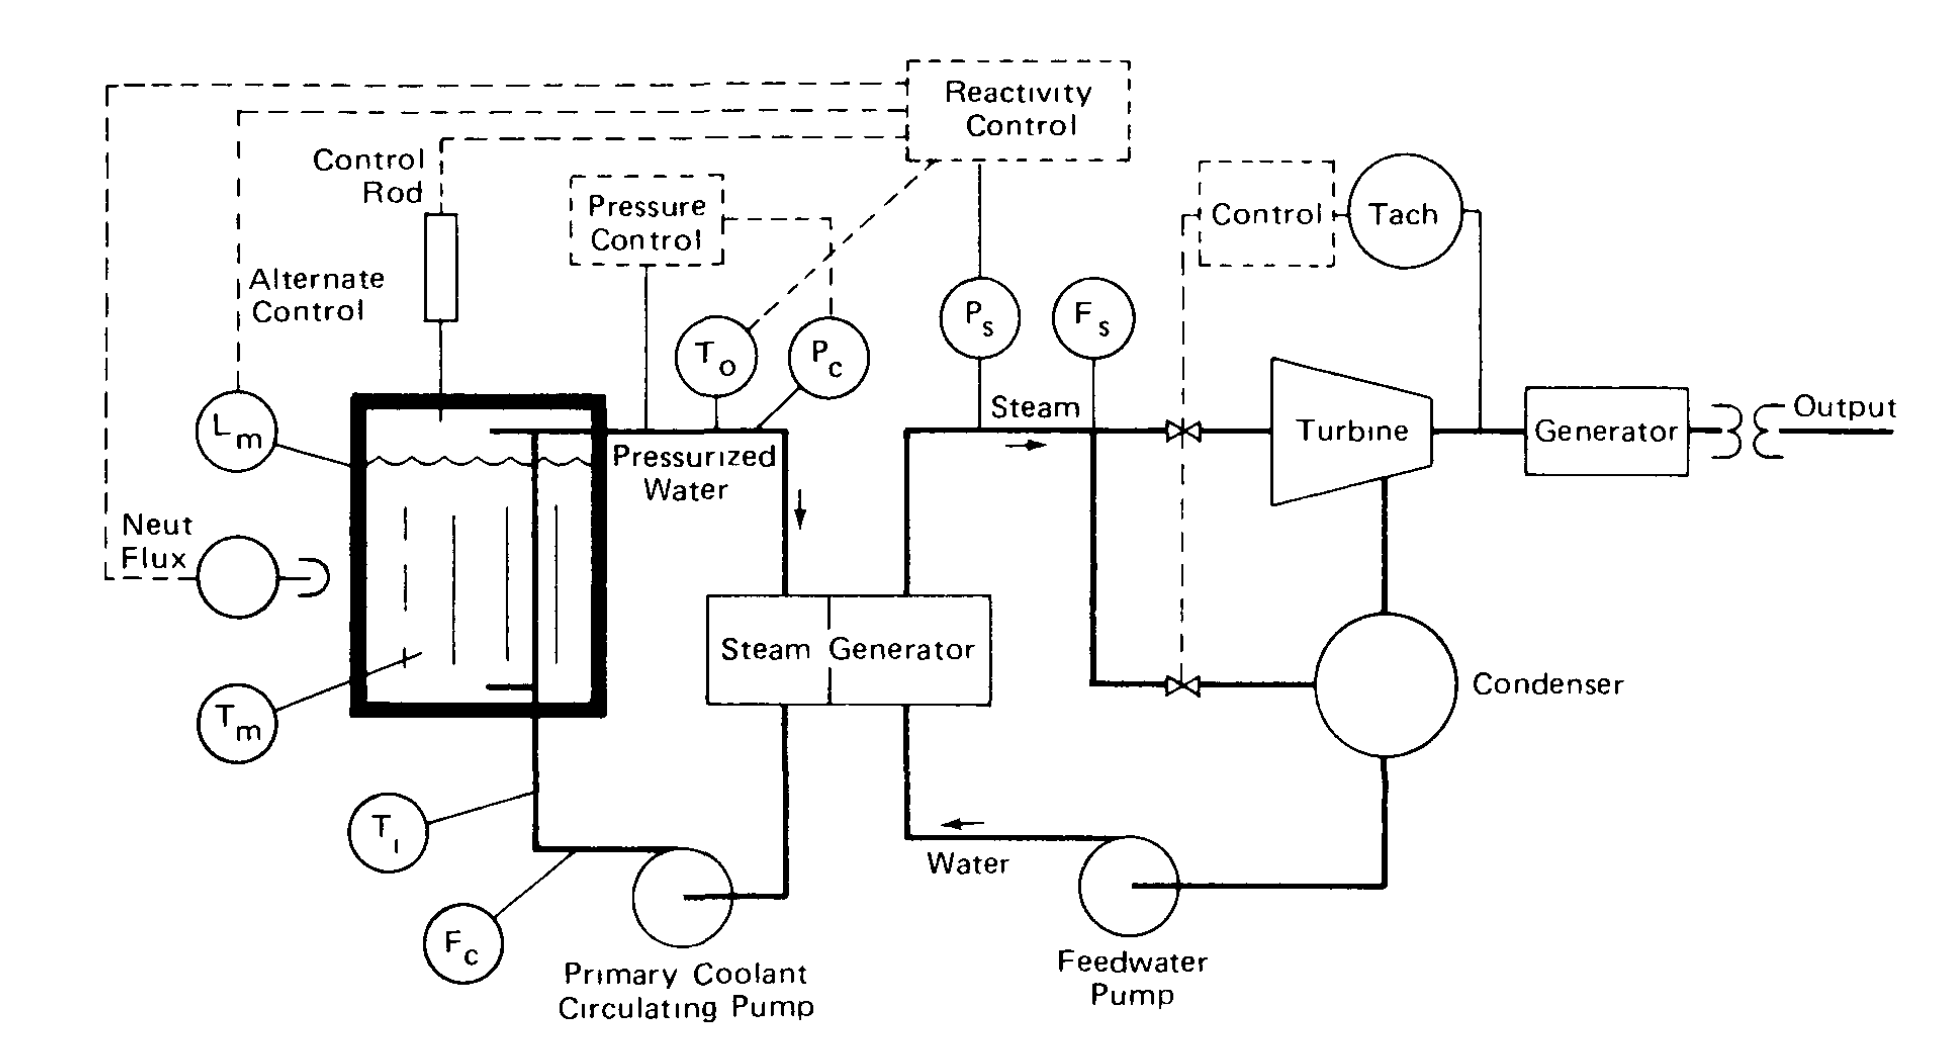
\includegraphics[width=\textwidth]{instrumentation.png}

    \column{0.48\textwidth}
    \begin{itemize}
      \item Pressurized Water Reactor (PWR)
      \item Boiling Water Reactor (BWR)
      \item Heavy Water Reactor (CANDU)
      \item Advanced Gas-cooled Reactor (AGR)
    \end{itemize}
  \note{
    Each design uses different coolants and moderators, which affect safety logic and monitoring strategies.\\
    PWRs are the most common worldwide. Sensors track neutron flux, coolant temperature, rod position, pressure, and flow rate.
  }
  \end{columns}
\end{frame}

\begin{frame}{Automatic Protection Systems}
  \subsubsection*{SCRAMs and Interlocks}
  \begin{columns}
    \column{0.49\textwidth}
    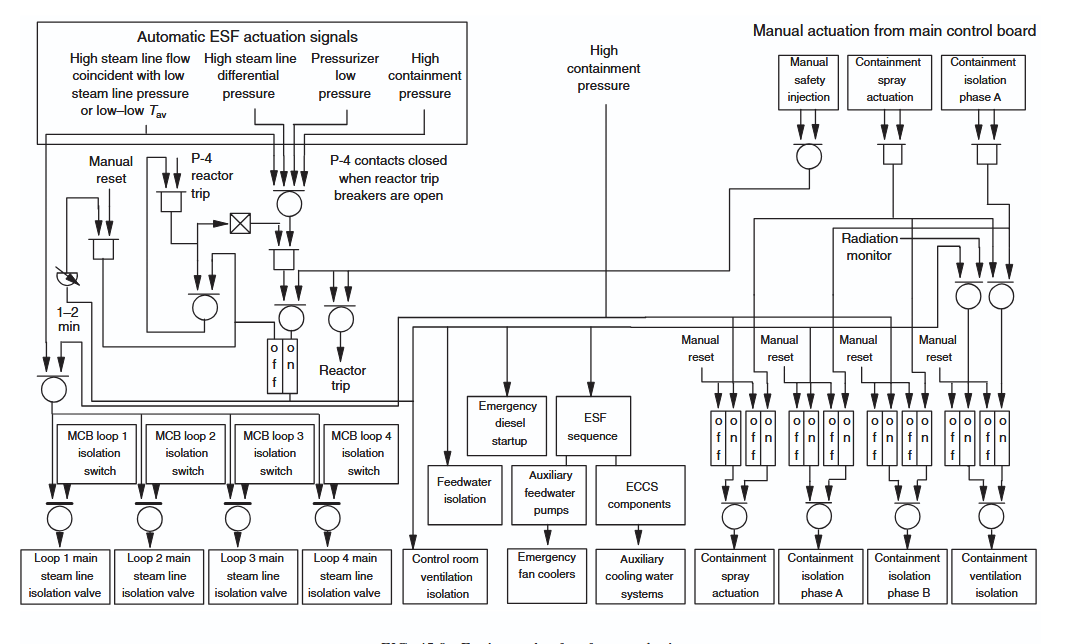
\includegraphics[width=0.95\textwidth]{safetylogic}

    \column{0.48\textwidth}
  \begin{itemize}
    \item Reactor protection systems (RPS): monitor reactivity, temperature, pressure
    \item Logic interlocks: prevent unsafe configurations
    \item Hardwired paths with digital backups
  \end{itemize}
  \note{Even the best operator can’t always react fast enough. That’s where automatic systems step in. SCRAMs instantly insert control rods. Protection logic compares real-time data to safety limits, triggering shutdowns, alarms, or backup actuation.}
\end{columns}
\end{frame}

\section{Broader Impacts}
\subsection{Historical Accidents: The Environmental Impact}
\begin{frame}{SL-1: Prompt Critical Accident}
  \begin{columns}
    \column{0.48\textwidth}
  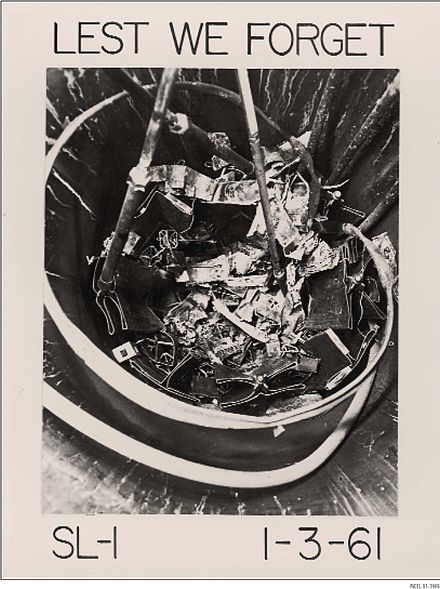
\includegraphics[width=\textwidth]{sl1diagram.jpg}

  \column{0.48\textwidth}
  \begin{itemize}
    \item Occurred January 3, 1961 in Idaho Falls.
    \item A single control rod was withdrawn manually beyond safe limits.
    \item Caused an instantaneous power excursion and steam explosion.
    \item All three operators died; first fatal U.S. nuclear accident.
  \end{itemize}
  \note{Local firefighters arrived in response to a fire alarm and found the facility abandoned.
Coffee cups remained warm, and food was left uneaten. As radiation alarms activated on their
dosimetry equipment, they realized a serious radiological event had occurred. Two operators
were located dead from radiation exposure. The third, Richard Legg, was discovered impaled
and pinned to the containment ceiling by a control rod—ejected upward during the reactor’s
prompt critical event.}
\end{columns}
\end{frame}


\begin{frame}{Three Mile Island: Partial Core Meltdown}
  \begin{columns}
    \column{0.48\textwidth}
  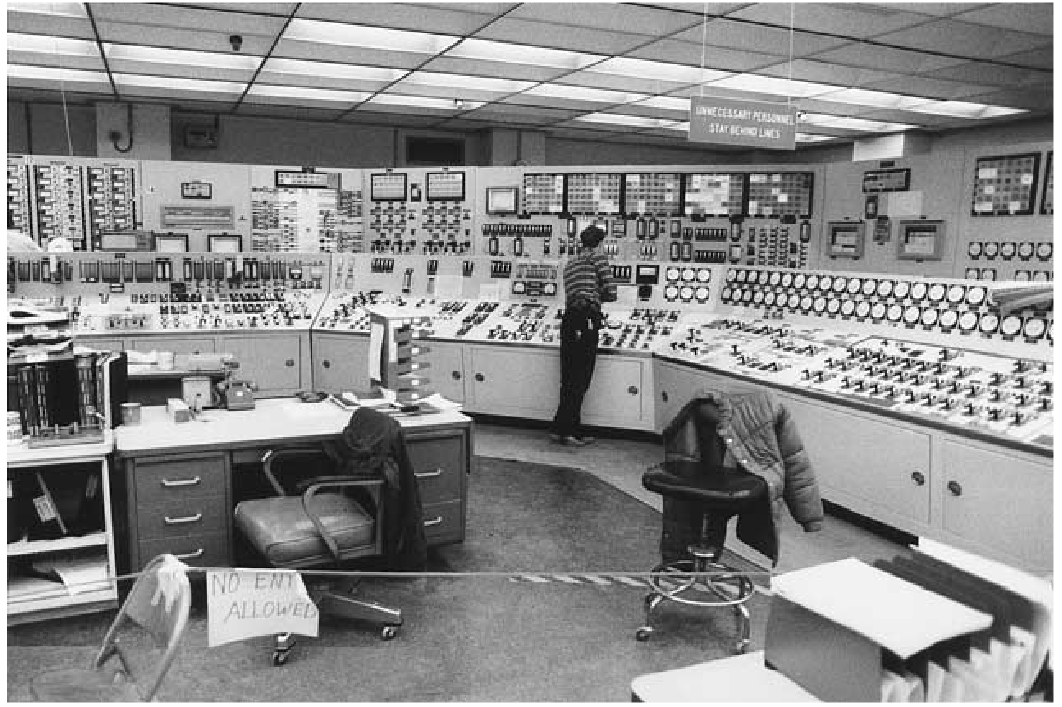
\includegraphics[width=\textwidth]{tmicontrolroom.png}

\column{0.48\textwidth}
  \begin{itemize}
    \item March 28, 1979 in Pennsylvania.
    \item Equipment failure: relief valve stuck open.
    \item Operator misinterpretation led to coolant pump shutdown.
    \item Reactor overheated—partial meltdown of core.
  \end{itemize}
\end{columns}

  \note{The Three Mile Island Unit 2 (TMI-2) accident occurred on March 28, 1979, near Harrisburg,
Pennsylvania, and remains the most serious commercial nuclear accident in the United States.
It was precipitated by the failure of a pressure-operated relief valve (PORV) that became
stuck open during a minor malfunction. The valve allowed coolant to escape from the
pressurizer, but due to inadequate instrumentation, operators believed it had closed properly}
\end{frame}

\begin{frame}{Chernobyl: Uncontrolled Power Surge}
  \begin{columns}
    \column{0.48\textwidth}
  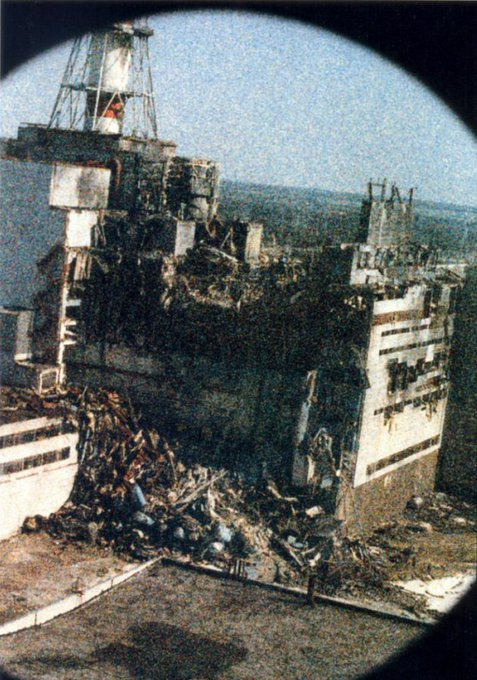
\includegraphics[width=\textwidth]{chernobylafter.jpg}
\column{0.48\textwidth}
  \begin{itemize}
    \item April 26, 1986 in Pripyat, USSR.
    \item Unsafe test conducted at low power with flawed RBMK reactor.
    \item Control rods exacerbated the surge due to graphite tips.
    \item Reactor exploded; massive radioactive release.
  \end{itemize}

  \note{The test intended to verify whether the rotational inertia
of the turbine could temporarily power the emergency coolant pumps in the event of a
grid power failure [7]. The RBMK-1000 reactor involved was a Soviet-designed graphite-
moderated, water-cooled system—flawed by both design and executionhe core overheated instantly, rupturing fuel channels and vaporizing coolant. A vi-
olent steam explosion lifted the reactor’s 2,000-ton upper biological shield. A second ex-
plosion—possibly from hydrogen or steam—further breached the structure and exposed the
graphite moderator, which caught fire. Figure 6 shows the aftermath of the explosion mere
hours after the explosion. The fire lofted radioactive particles into the upper atmosphere,
affecting much of Europe }
\end{columns}
\end{frame}

\begin{frame}
  \centering
  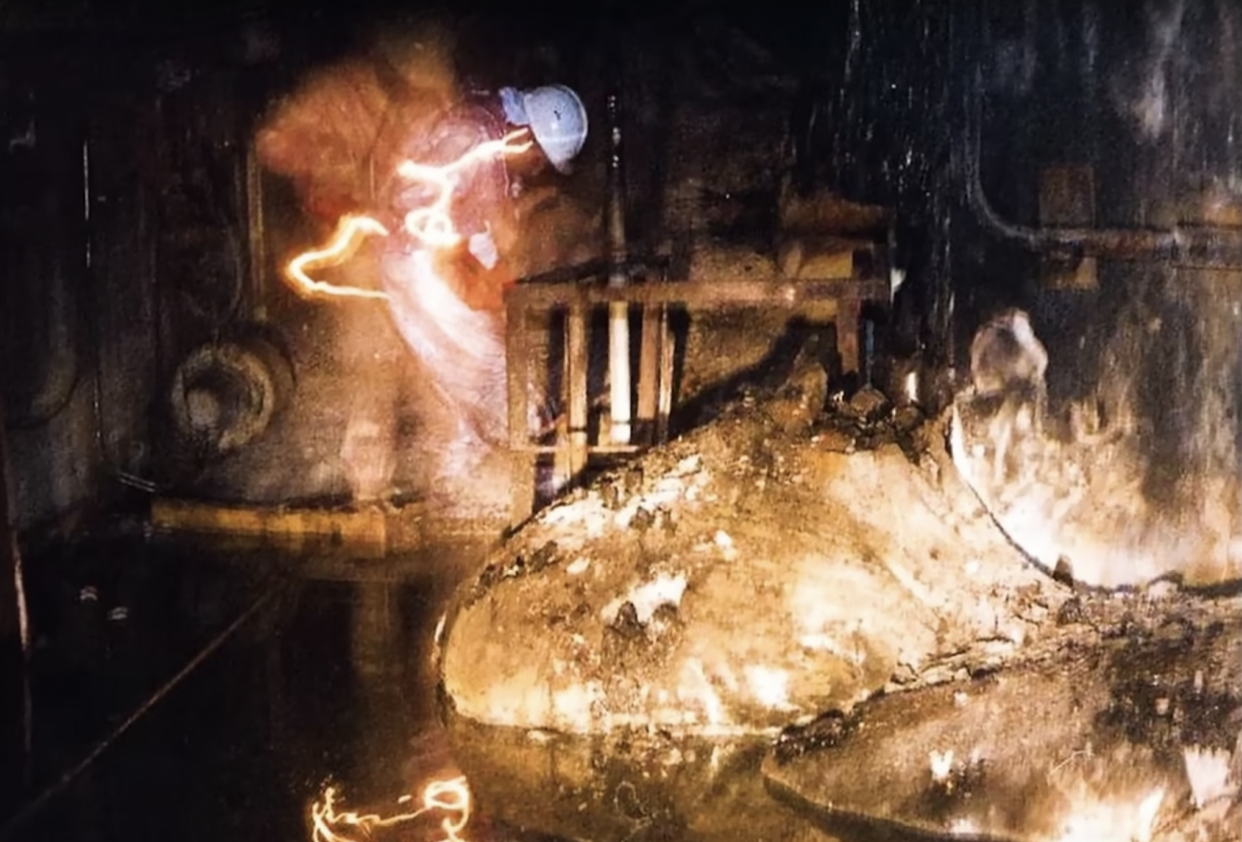
\includegraphics[width=0.65\textwidth]{elephantsfoot.png}
  \note{The aftermath of Chernobyl catalyzed global reevaluation of nuclear safety, reactor de-
sign, and operator training. The international community pushed for increased transparency,
safety audits, and enhanced containment strategies. The photograph in Figure 7 famously
shows the “Elephant’s Foot,” a deadly corium formation. The strange visual static in the
image is not lightning, but film degradation from intense radiation—testament to the un-
precedented radioactive environment at the site}
\end{frame}

\begin{frame}{Fukushima Daiichi: Station Blackout}
  \begin{columns}
    \column{0.48\textwidth}
  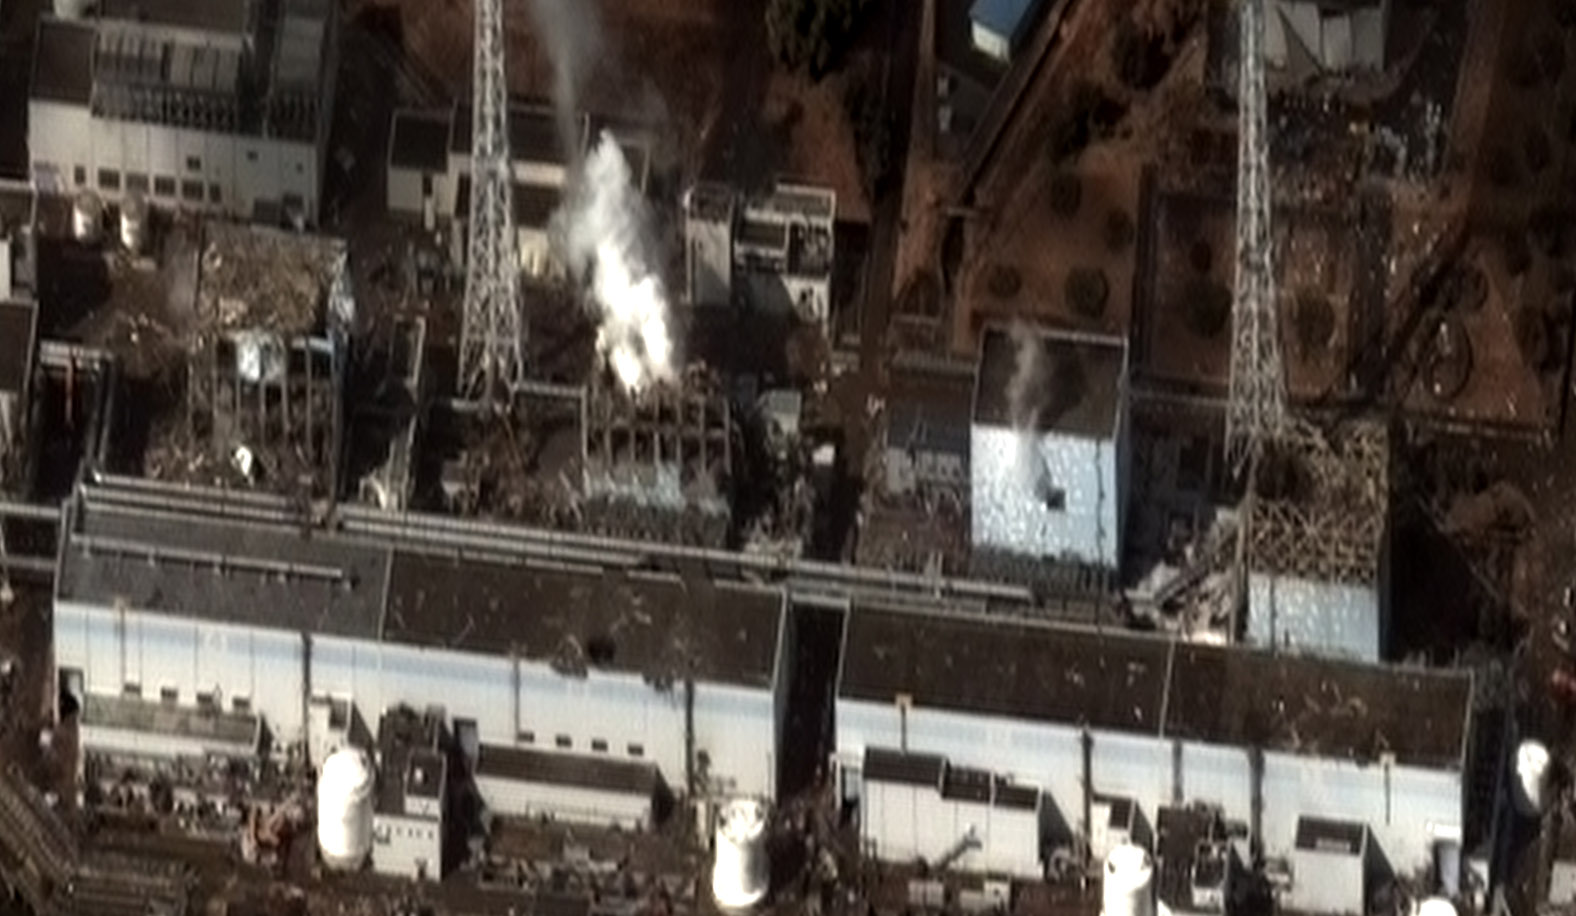
\includegraphics[width=\textwidth]{fukushimaafter.jpg}
  \column{0.48\textwidth}
  \begin{itemize}
    \item March 11, 2011 in Japan.
    \item Magnitude 9.0 earthquake triggered tsunami.
    \item Backup diesel generators flooded—loss of core cooling.
    \item Hydrogen buildup led to explosions in three reactors.
  \end{itemize}
  \note{The Fukushima-Daiichi Nuclear Power Station, operated by TEPCO, was critically
affected. Although the three operating reactors—Units 1, 2, and 3—successfully SCRAMed
(shut down automatically), the tsunami flooded the site and disabled both the offsite grid
connections and emergency diesel generators [12]. This unprecedented loss of power across all
units is illustrated in Figure 8, which shows the reactor buildings after successive hydrogen
explosions.}
\end{columns}
\end{frame}

\subsection{Technological Impact}
\begin{frame}{Human Operators: Essential Links}
  \begin{columns}
    \column{0.48\textwidth}
  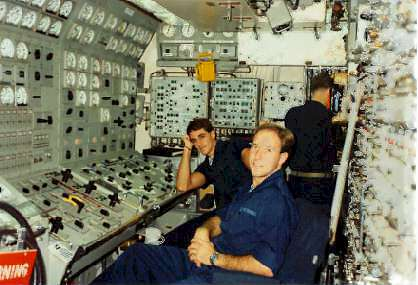
\includegraphics[width=\textwidth]{maneuvering-watch.jpg}
    \note{Human operators are the last line of defense. They interpret complex data, make decisions under pressure, and ensure systems operate safely. The operators in this picutre are in a room named maneuvering. In this tight cramped space, you can see the control panel to control the reactor, and further back the electric plant control panel of a S5W reactor powered ship.}

    \column{0.48\textwidth}
    \begin{itemize}
      \item Operators monitor instrumentation and respond to alarms.
      \item They must understand system behavior and safety limits.
      \item Training and vigilance are critical for safe operation.
    \end{itemize}
  \end{columns}
\end{frame}

\begin{frame}{Human Factors Engineering}
  \begin{columns}
    \column{0.48\textwidth}
  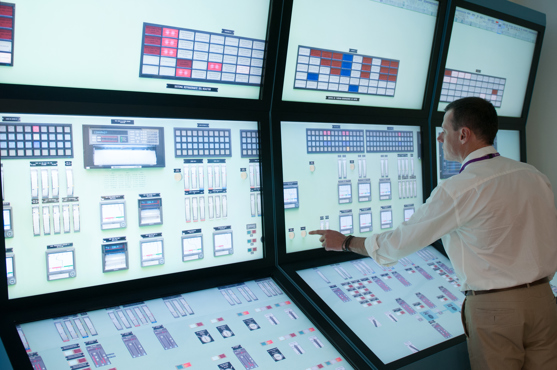
\includegraphics[width=\textwidth]{simulators.jpg}
  \column{0.48\textwidth}
  \begin{itemize}
    \item Post-TMI, HFE became a formal discipline in nuclear plant design.
    \item Goals: reduce confusion, prevent overload, clarify alarms.
    \item INPO and NRC led redesigns of control interfaces.
  \end{itemize}
  \note{Human-machine interface redesign became essential after TMI. Alarm logic, indicator layout, and system feedback were all reengineered. The need to provide complex and realistic simulation training for operators has increased tenfold since the 1980s.}
\end{columns}
\end{frame}

\begin{frame}{Ethical Oversight in Automation}
  \begin{columns}
    \column{0.48\textwidth}
  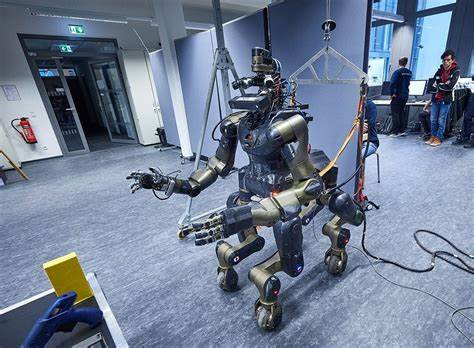
\includegraphics[width=\textwidth]{ethicaldesign.jpg}
  \column{0.48\textwidth}
  \begin{itemize}
    \item Systems must support—not replace—human oversight.
    \item Overreliance on automation can erode accountability.
    \item Ethical design considers failure modes, transparency, and operator input.
  \end{itemize}
  \note{Designing for ethical oversight means respecting human limits while reinforcing responsibility. The worst outcomes often arise when operators are sidelined.}
\end{columns}
\end{frame}


\subsection{The Societal Impact of Nuclear Power}
\begin{frame}{Why Nuclear Declined}
  \subsubsection*{Societal Impact: Policy, Perception, and Paralysis}
  \begin{itemize}
    \item Each accident—from SL-1 to Fukushima—prompted strict new regulations.
    \item Longer licensing cycles delayed new builds by decades.
    \item Public opposition and fear, not technical failure, stalled the industry.
    \item Skilled labor and supply chains diminished as construction halted.
  \end{itemize}
  \note{The world walked away not because nuclear failed—but because faith in its management eroded. Regulation became slower, and expertise drifted away.}
\end{frame}
\subsection{The Economic Impact}
\begin{frame}{Challenges Today}
  \begin{itemize}
    \item Most operating reactors in the U.S. are past mid-life.
    \item Replacing the aging nuclear workforce is a growing challenge.
    \item Engineering firms that once supported nuclear have pivoted to renewables.
    \item Safety margins remain—but the supporting infrastructure has weakened.
  \end{itemize}
  \note{Many of the companies and capabilities that built the first generation of plants no longer exist in their original form. As a result, the ability to construct new certified plants has greatly diminished. The nuclear industry is now at a crossroads, where the lessons of the past must inform the future.}
\end{frame}

\section{Conclusion}

\begin{frame}{Conclusion: A Deliberate Future}
  \begin{columns}
    \column{0.45\textwidth}
    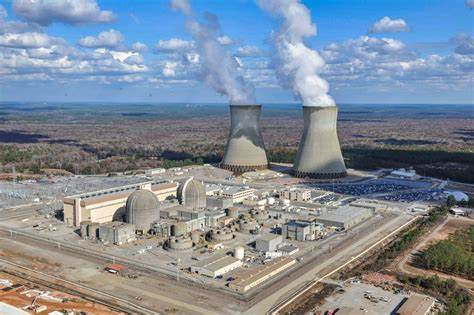
\includegraphics[width=\textwidth]{vogtle}
    \note{The future of nuclear power depends on our ability to learn from the past, innovate responsibly, and rebuild trust.}

    \column{0.55\textwidth}
    \begin{itemize}
      \item Nuclear power is safe when designed, operated, and overseen with care.
      \item Instrumentation and human oversight must evolve together.
      \item Ethical design puts operators in control, not out of the loop.
      \item The tools are available, what remains is the will to rebuild trust.
    \end{itemize}
  \end{columns}
\end{frame}

\begin{frame}{Conclusion: A Deliberate Future}
  \begin{itemize}
    \item Nuclear safety is engineered, not assumed.
    \item Instrumentation and human oversight must evolve together.
    \item Ethical design puts operators in control, not out of the loop.
    \item The tools are available—what remains is the will to rebuild trust.
  \end{itemize}
  \note{Safe nuclear power isn’t an inevitability—it’s a discipline. What matters is not just how reactors are built, but how they are overseen.}
\end{frame}

\end{document}
